\documentclass[
11pt,%
tightenlines,%
twoside,%
onecolumn,%
nofloats,%
nobibnotes,%
nofootinbib,%
superscriptaddress,%
noshowpacs,%
centertags]%
{revtex4}
\usepackage{ljm}
\usepackage{listings}
\usepackage{amsmath}

\lstset{
language=C++,
basewidth=0.5em,
xleftmargin=45pt,
xrightmargin=45pt,
basicstyle=\small\ttfamily,
keywordstyle=\bfseries\underbar,
numbers=left,
numberstyle=\tiny,
stepnumber=1,
numbersep=10pt,
showspaces=false,
showstringspaces=false,
showtabs=false,
frame=trBL,
tabsize=2,
captionpos=t,
breaklines=true,
breakatwhitespace=false,
escapeinside={\%*}{*)}
}

\begin{document}

\titlerunning{Scaling of supercomputer calculations}
\authorrunning{Shabanov et al.}

\title{Исследование эффективности масштабирования суперкомпьютерных вычислений на неструктурированных поверхностных расчетных сетках}

\author{\firstname{B.~M.}~\surname{Shabanov}}
\email[E-mail: ]{shabanov@jscc.com}
\affiliation{Joint Supercomputer Center of the Russian Academy of Sciences -- branch of Scientific Research Institute of System Analysis of the Russian Academy of Sciences, Leninsky prospect 32a, Moscow, 119334, Russia}

\author{\firstname{A.~A.}~\surname{Rybakov}}
\email[E-mail: ]{rybakov.aax@gmail.com}
\affiliation{Joint Supercomputer Center of the Russian Academy of Sciences -- branch of Scientific Research Institute of System Analysis of the Russian Academy of Sciences, Leninsky prospect 32a, Moscow, 119334, Russia}

\author{\firstname{S.~S.}~\surname{Shumilin}}
\email[E-mail: ]{shumilin@jscc.com}
\affiliation{Joint Supercomputer Center of the Russian Academy of Sciences -- branch of Scientific Research Institute of System Analysis of the Russian Academy of Sciences, Leninsky prospect 32a, Moscow, 119334, Russia}

\author{\firstname{M.~Yu.}~\surname{Vorobyov}}
\email[E-mail: ]{nordmike@jscc.com}
\affiliation{Joint Supercomputer Center of the Russian Academy of Sciences -- branch of Scientific Research Institute of System Analysis of the Russian Academy of Sciences, Leninsky prospect 32a, Moscow, 119334, Russia}

\firstcollaboration{(Submitted by A.~M.~Elizarov)} % Add if you know submitter.
%\lastcollaboration{ }

\received{TODO}

\begin{abstract}
When solving complex problems of numerical modeling, computational grids, containing hundreds of millions of cells are quite often.
Modern tasks even cross the line of billion cells.
Workstations are unable to cope with such volume of data and computation.
To perform computations of this volume we need to use supercomputer clusters consisting of many computational nodes interconnected by a high-speed communication network.
In this case, it is necessary to perform the decomposition of the computational grid into separate domains in order to ensure its parallel processing on all nodes of the cluster.
These domains are distributed among the computational nodes of the supercomputer and are processed independently of each other.
To synchronize computations, after each iteration of cell processing, data exchanges are performed at the boundaries between adjacent contiguous domains.
To efficiently perform computations and scale them to a large number of computational nodes, it is necessary to develop efficient algorithms for decomposition of computational grids that generate many domains with imposed requirements.
This requirements include: number of cells, uniformity of cells' distribution over domains, domain connectivity and the size of boundaries between them.
At the same time, theoretical indicators of the efficiency of decomposition of computational grid do not guarantee the efficient execution of a real problem on a supercomputer.
We consider a hierarchical decomposition algorithm with the choice of the optimal criterion for dividing grid into domains.
As such a grid we study an unstructured surface mesh used to calculate the processes of interaction of a volumetric body with the environment.
Using this decomposition algorithm, supercomputer calculations are performed on the computing resources of JSCC RAS in order to measure the practical indicators of scalability of highly loaded applications.
\end{abstract}

\subclass{65Y05,65Y20,49M27} % Enter 2010 Mathematics Subject Classification.

\keywords{суперкомпьютер, поверхностная неструктурированная расчетная сетка, декомпозиция, домен, высокопроизводительные вычисления, масштабирование вычислений}

\maketitle

\section{Introduction}

Modern computational applications are extremely demanding on computational resources.
For large tasks it is not possible to execute them on a separate computer (one microprocessor or one server) in reasonable time.
There is a need to use supercomputer clusters for computations, consisting of many computational nodes.
In order to perform a task on a supercomputer, it is necessary to divide its computational domain into separate subdomains and process them in parallel.
To improve the efficiency of supercomputer applications within a computing node, various methods of data preparation and parallelization of execution for systems with shared memory are used.
Low-level optimizations of program code, such as vectorization, which can significantly increase the speed of application execution can also be very efficient.
Of course, at the boundaries of domain contact, it becomes necessary to synchronize computations, which is achieved by data exchange (for example, using MPI).
Thus, the execution of supercomputer calculations consists of two alternating steps: parallel processing of cells of the computational domain and data exchange at the boundaries of contact of domains.
The efficiency of supercomputer applications execution essentially depends on the quality of the computational grid decomposition and its distribution over different computational nodes.

This article is devoted to the problem of decomposition of a surface unstructured computational grid for distribution between the nodes of a homogeneous supercomputer cluster  to increase the efficiency of computational scaling.
By homogeneous we mean a cluster consisting of the same computational nodes.
Take a surface mesh consisting of $ S $ computational cells, let the supercomputer consist of $ n $ computational nodes with the same characteristics.
We will also assume that the speed of data exchange between any two computational nodes is the same for all nodes.
Extension of the problem of distributing the computational load to a heterogeneous computational cluster is achieved by entering weights for computational nodes and for data exchange channels, as described in [TODO].
If we represent the processing speed of computational cells on one computational node as $ a^{-1} $, then the execution time of one iteration of computations on one computational node will be equal to $ T_1 = aS $.
Now let the computational domain be divided into $ n $ domains each containing $ S_i $ cells ($ i = 1, n $).
Let us denote by $ L_{ij} $ the number of edges that form the border between the domains $ S_i $ and $ S_j $.
We will assume that each domain is processed on its own computational node.
Thus, all domains are processed in parallel, and the processing time for all cells is determined by the processing time for the largest domain.
In addition to processing all computational cells, after the calculation iteration, it is necessary to exchange data between all pairs of domains along their boundaries.
Let the speed of data transfer between nodes be determined by the value of $ b^{-1} $, and all exchanges are performed in parallel.
Then the execution time of all exchanges is determined by the time of data exchange across the longest boundary.
Based on this, it is possible to determine the total execution time of one iteration of calculation when executing on $ n $ computational nodes:

\begin{equation}
T_n = a \max_{i = 1,n}{S_i} + b \max_{i,j=1,n}{L_{ij}}.
\end{equation}

The criterion for optimization of computational grid's decomposition is the reduction of time for performing calculations, that is, the value of $ T_n $.
The calculation execution time directly depends on the size of the largest domain, however, we will consider not the absolute size of the domain, but its deviation from the theoretical optimal value.
Obviously, in the ideal case, during decomposition, all domains should have the size $ \frac{S}{n} $, and the relative deviation from the ideal size in percentage can be calculated by the formula:

\begin{equation}
D = 100 \% \left( \frac{n}{S} \max_{i=1,n}{S_i} - 1 \right).
\end{equation}

The second important criterion for the quality of the performed decomposition is the largest value of the length of the boundary between pairs of domains.
In this case, the absolute characteristic can be used, since the length of the boundary is rather difficult to predict, and generally speaking, it has no theoretical minimum.
Depending on the geometry of the grid under consideration, the length of the boundary between domains can theoretically be zero.
We will use the following value as a criterion for comparing various grid decomposition methods:

\begin{equation}
L = \max_{i,j=1,n}{L_{ij}}.
\end{equation}

Despite the fact that, in our assumptions, all data exchanges between domains are executed simultaneously, the total volume of all exchanges significantly affects the data exchange rate, so this parameter must also be taken into account.
Let us introduce it in the following form.
The total number of edges in the computational grid remains unchanged regardless of the decomposition algorithm and number of domains.
We denote the total number of edges in the grid by $ E $.
Among these edges there are border edges that have only one incident cell, their number is also constant and equal to $ E_B $ (from the word "border").
The rest of the edges have two incident cells.
If both cells incident to a certain edge belong to the same domain, then we call such an edge an inner edge of this domain
We denote their number by $ E_{INN} $ from the word "inner".
Otherwise the edge enters the boundary between two domains and we call it an interdomain edge.
$ E_{INT} $ is their number.
There can be no other types of edges.
Thus, the relation $ E = E_B + E_{INN} + E_{INT} $ is fulfilled.
As a parameter for evaluating the quality of decomposition, we will consider the fraction of interdomain edges in the total number of mesh edges, that is, the value:

\begin{equation}
I = 100 \% \left( \frac{E_{INT}}{E} \right)
\end{equation}

To assess the quality of the computational mesh decomposition, all three described parameters should be taken into account: $ D $ is the deviation of the biggest domain size from the ideal value, $ I $ is the fraction of interdomain edges in the total number of edges of the computational mesh, and $ L $ is the length of the longest boundary between pairs of domains.
The lower the values of these criteria, the better the decomposition is and the more efficient calculations can be expected when running on a real machine.

\section{Распараллеливание вычислений на неструктурированной расчетной сетке}

\begin{figure}[h]
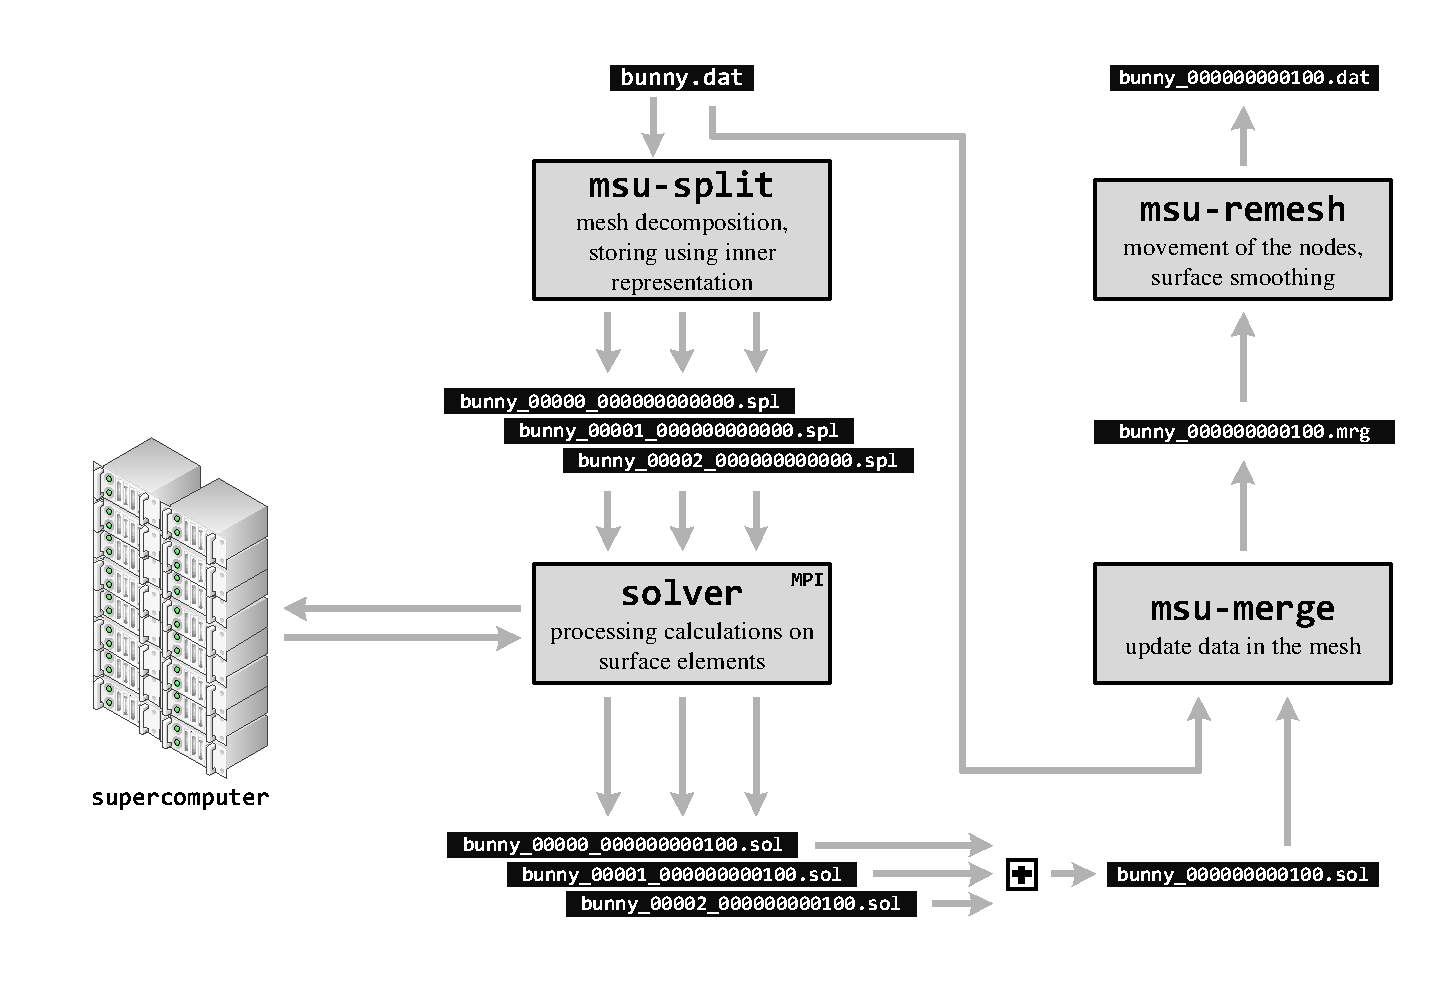
\includegraphics[width=1.0\textwidth]{pics/02-scheme.pdf}
\captionstyle{center}\caption{Схема распараллеливания вычислений на суперкомпьютере.}\label{fig:02-scheme}
\end{figure}

Consider a parallelization scheme for computations associated with modeling the interaction of a volumetric body with the environment.
In this case, calculations are carried out on the surface of an interacting body described by an unstructured surface computational grid (GSU - Grid Surface Unstructured) with triangular cells.
In the considered calculation scheme on the body surface, various physical processes are considered, including surface deformation, the flow of a liquid film, and ice accretion, which ultimately should lead to remeshing of the calculated surface.
The calculation scheme is thus divided into several independent functional modules (the scheme of interaction of the modules is shown in Fig~\ref{fig:02-scheme}.

The first module -- \texttt{gsu-split} -- is designed to load the computational mesh, decompose it into several domains and prepare it for solver.
The physical solver \texttt{solver} is intended only for high-load computations, it interacts with the supercomputer cluster and operates on an arbitrary number of computational nodes.
This is the most resource-demanding part of the application, which takes more than 90 \% of the estimated time, so it is implemented using MPI, OpenMP and vectorization of the program code.
After carrying out the necessary calculations, the \texttt{solver} module returns the accumulated calculated data from different time points, which are fed into the \texttt{gsu-merge} data fusion module.
The last link in the chain of calculations is the \texttt{gsu-remesh} module, which receives a computational grid as input (in general case, a set of computational grids from different points in time) and remeshes it.

\section{Decomposition of an unstructured computational grid}

[TODO] describes a parallel algorithm for geometric decomposition of grid data.
During the operation of this algorithm, the current domain is sequentially halved using a plane section.
According to the logic of this algorithm, the initial head domain (\texttt{h} -- head) is halved into a pair of domains \texttt{hl} (left), \texttt{hr} (right), each of which is further halved, and so on up to any number of domains equal to a power of two.

We propose to extend this algorithm by introducing arbitrary criteria for dividing the current domain into a pair of smaller domains.
First, consider the scheme of simple division of a domain in half using an arbitrary criterion by which the division is performed (Fig.~\ref{fig:03-split}).

\begin{figure}[h]
\includegraphics[width=1.0\textwidth]{pics/03-split.pdf}
\captionstyle{center}\caption{A scheme of halving the domain according to the selected attribute fun.}\label{fig:03-split}
\end{figure}

Assume a set of cells of domain \texttt{h} and some function \texttt{fun} for extracting the feature from a cell.
The first step is to calculate the set of features for all cells (\texttt{s} -- signs):
\begin{equation*}
	s = \{fun(h_i)~|~h_i \in h\}.
\end{equation*}

Sort \texttt{s}.

In the sorted set of features, the median value should be chosen (\texttt{b} -- blade):
\begin{equation*}
	b = median(s).
\end{equation*}

This value will be used to split the domain into two smaller domains (\texttt{hl} -- head left, \texttt{hr} -- head right) using two simple filters:
\begin{equation*}
	hl = \{h_i~:~fun(h_i) < b,~h_i \in h\},
\end{equation*}
\begin{equation*}
	hr = \{h_i~:~fun(h_i) \geq b,~h_i \in h\}.
\end{equation*}

After splitting a domain into two smaller domains, you can calculate a parameter that reflects the efficiency of splitting.
We propose to use the length of the boundary between the two newly formed domains as such a parameter.
Thus, the splitting criterion depends on the function of calculating the attribute \texttt{fun}.
In turn, this means that when performing a partition, it is not necessary to be limited to one function of calculating a feature.
Instead, you can submit a list of functions, for each function calculate the parameter of quality of the partition and, as a result, stop at the function, which ultimately leads to the most efficient partition.
If we simply use the extraction of the three coordinates of the cells' centers as functions for calculating the feature of a cell, then we will obtain in its pure form an algorithm for the geometric decomposition of the grid with the choice of longest coordinate for splitting.
The results of applying this algorithm can be seen in Fig.~\ref{fig:03-explode-bunny} and Fig.~\ref{fig:03-hierarch}.

\begin{figure}[h]
\includegraphics[width=1.0\textwidth]{pics/03-explode-bunny.pdf}
\captionstyle{center}\caption{An example of decomposition of a surface computational grid using a hierarchical algorithm.}\label{fig:03-explode-bunny}
\end{figure}

\begin{figure}[h]
\includegraphics[width=1.0\textwidth]{pics/03-hierarch.pdf}
\captionstyle{center}\caption{Examples of surface computational grid decomposition using a hierarchical algorithm.}\label{fig:03-hierarch}
\end{figure}

By varying the set of features for calculating features by which the domain can be partitioned, it is possible to perform geometric decomposition along the direction of any curve for which the cell projection is calculated.
Decomposition using this method is not limited to geometric features only.
Features calculation functions can be used to analyze the physical data of cells, for example, to localize and isolate areas with increased pressure into separate domains.
Within the framework of this work, the described algorithm for decomposition of the surface unstructured computational grid was applied to the surface grids used to calculate the icing of the aircraft surface.
When calculating the icing of an aircraft, the bulk of the computations relates to the processing of surface cells.
Shared data between adjacent domains is collected on interdomain edges.
The typical size of such grids was about $ 10^5 $ cells. We considered both simply connected and not simply connected surfaces, as well as surfaces consisting of several zones isolated from each other.

It should be noted that the theoretical quality parameters $ D $, $ L $, $ I $ are quite low.
The $ D $ parameter is practically zero, since at each step the domain is divided strictly in half.
The deviations in the lengths of the boundaries between domains and the total length of the boundaries are also acceptable, despite the fact that the algorithm does not guarantee the formation of domains with minimal boundaries or even connected domains
In the worst cases, domains of arbitrary shape and consisting of an arbitrary number of isolated parts of the surface may arise.
Of course, a significant limitation of the algorithm is that it can be used to partition the surface only into the number of parts, which is a power of two, but the close-to-zero value of the computational load balancing quality index $ D $ allows in this case to neglect this drawback.

\section{Organization of interprocess exchanges}

\begin{figure}[h]
\includegraphics[width=1.0\textwidth]{pics/04-MPI.pdf}
\captionstyle{center}\caption{Scheme of execution of MPI-exchanges across the border of two zones.}\label{fig:04-MPI}
\end{figure}

When performing calculations on a decomposed grid, at each iteration of the computation, it is necessary to exchange data at each boundary between domains.
In our case, when performing the decomposition of the computational grid, the boundary between two domains is represented by an arbitrary set of interdomain edges.
In this case, the boundary may be discontinuous, it may even consist of separate edges, therefore the sequence of interdomain edges is not important when describing the boundary.

Fig.~\ref{fig:04-MPI} shows a scheme of organization of interprocess exchanges.
Two domains (we will conventionally call them left and right), processed in MPI processes numbered 0 and 1, are separated by a boundary consisting of three edges.
In this case, there are three cells in the left domain that are adjacent to the considered boundary, in the right domain there are only two such cells (since cell 23R is adjacent to two edges of the boundary at once).
To organize interprocess communications in each domain, ghost cells are created for each edge of the considered boundary, which are involved in calculating flows through the edges.
At the same time, there is no need to recalculate physical values in ghost cells
All data for ghost cells is obtained using MPI exchanges from real cells of a neighboring domain.

To transfer data from the real border cells of the domain to the ghost cells of the neighboring domain, buffers for sending and receiving data are organized in each of the two neighboring domains.
The data exchange sequence is as follows (the diagram is shown in Fig.~\ref{fig:04-MPI}).
First, data from real boundary cells is written to the corresponding send buffers (send buff), then asynchronous commands \texttt{MPI\_Irecv} for receiving messages in the data receiving buffers (recv buff) are executed for all boundaries of the computational grid.
After that, commands for asynchronous sending of data \texttt{MPI\_Isend} from the send buffers are also executed simultaneously for all boundaries of the computational grid.
Next, it waits for the completion of all asynchronous data exchanges using the \texttt{MPI\_Waitall} function.
The last step, completing the exchange of data between neighboring domains, is the transfer of the received physical values from the data receiving buffers (recv buff) to the corresponding ghost cells.

Note that some data duplication may occur when using ghost cells.
For example, in the presented diagram, cell 23R from the right domain corresponds at once to two ghost cells in the left domain.
These cells contain the same data.
This duplication of information is acceptable, since the data of the ghost cells is used only for reading to perform the calculation of flows across the domain boundary, therefore, in this case, there is no need to perform any synchronization of the same ghost cells.

\section{Efficiency of scaling supercomputer computations}

Для замеров показателей масштабируемости вычислений на неструктурированной поверхностной расчетной сетке была использована тестовая поверхность обтекаемого трехмерного тела, содержащая порядка $2 \cdot 10^5$ узлов и $4 \cdot 10^5$ ячеек.
В ячейках выполнялись расчеты, связанные с моделирование течения жидкой пленки, решением уравнений теплового баланса на поверхности, а также перестроение и сглаживание поверхности.
Для декомпозиции поверхностной сетки использовался простой иерархических алгоритм деления доменов пополам, описанный в данной статье, в котором в качестве признаков ячеек брались три координаты центра.
При этом в результате критерием выбора конкретной координаты для деления домена являлась минимизация длины границы между двумя доменами (такой подход позволяет выполнять деление домена по наиболее протяженному направлению).

\begin{table}[!h]
\label{tbl:supercomputers}
\setcaptionmargin{0mm}
\onelinecaptionsfalse
\captionstyle{flushleft}
\caption{Конфигурации сегментов суперкомпьютера МВС-10П ОП, на которых производились замеры масштабирования вычислений.}
\bigskip
\begin{tabular}{|c|c|c|c|c|}
\hline
\parbox{3.5cm}{\textit{Семейство\\микропроцессоров Intel}} & \parbox{4.0cm}{\textit{Количество\\процессоров / ядер /\\потоков в узле}} & \parbox{3.0cm}{\textit{Частота\\микропроцессора}} & \parbox{3.0cm}{\textit{Объем\\оперативной\\памяти в узле}} & \parbox{2.0cm}{\textit{Поддержка\\AVX-512}} \\
\hline
Xeon Broadwell & 2 / 32 / 64 & 2.6 GHz & 128 GB & no \\
\hline
Xeon Phi KNL & 1 / 72 / 288 & 1.5 GHz & 96 GB & yes \\
\hline
Xeon Skylake & 2 / 36 / 72 & 3.0 GHz & 192 GB & yes \\
\hline
Xeon Cascade Lake & 2 / 48 / 96 & 3.0 GHz & 192 GB & yes \\
\hline
\end{tabular}
\label{tab:supercomputers}
\end{table}   

Для измерения показателей масштабируемости вычислений использовались гомогенные сегменты вычислительной системы Межведомственного суперкомпьютерного центра РАН.
Всего расчеты проводились на четырех вычислительных сегментах, характеристики узлов которых приведены в таблице \ref{tab:supercomputers}.
В данной таблице можно отметить, что все микропроцессоры кроме Xeon Broadwell поддерживают набор инструкций AVX-512, позволяющий использовать специальные 512-битные векторные регистры для эффективной векторизации кода.
Также следует выделить вычислительные узлы на базе микропроцессора Xeon Phi KNL.
Эти микропроцессоры отличаются огромным количеством вычислительных ядер, каждое из которых способно выполнять до 4 потоков, что позволяет эффективно распараллеливать расчетные приложения вплоть до 288 потоков на одном микропроцессоре.

\begin{figure}[h]
\includegraphics[width=0.8\textwidth]{pics/speedup.pdf}
\captionstyle{center}\caption{Ускорение вычислений на суперкомпьютерах МСЦ РАН при увеличении количества узлов.}\label{fig:speedup}
\end{figure}

Основной целью выполняемых запусков было проведение замеров показателей сильной масштабируемости вычислений при полном распараллеливании внутри вычислительных узлов с использованием OpenMP.
То есть для всех запусков использовалась одна и та же поверхность (которая дробилась на нужное количество вычислительных узлов), а также в расчетах были задействованы все потоки, доступные внутри вычислительных узлов. 

При проведении расчетов замеры выполнялись независимо для каждой вычислительной системы в отдельности.
Приведем описание измеряемых величин в процессе расчета для одной конкретной вычислительной системы.
В качестве эталонного времени использовалось время выполнения задачи на одном вычислительном узле: $t(1)$.
Также были выполнены замеры времени выполнения задач для количества вычислительных узлов, равного степени двойки (2, 4, 8, 16, 32, 64).
При этом ускорением на количестве узлов, равном $i$, считалось значение величины $s(i) = \frac{t(1)}{t(i)}$.
На Fig.~\ref{fig:speedup} приведены диаграммы ускорения вычислений при увеличении количества вычислительных узлов для разных вычислительных систем.

Кроме вычисления непосредственно ускорения выполнения кода производились расчеты эффективности масштабирования.
Под эффективности масштабирования вычислений в данном случае понимается величина $e(i) = \frac{s(i)}{i}$.
Физический смысл данного показателя заключается в следующем.
Можно считать, что в случае идеального распараллеливания вычислений при увеличении количества вычислительных узлов в $n$ раз время выполнения уменьшается ровно в $n$ раз.
Таким образом в случае идеального распараллеливания $s(i) = i$, а $e(i) = 1$.
Эффективность масштабирования вычислений является удобным индикатором качества создания исполняемого параллельного кода и сравнения между собой различных вычислительных систем.
Заметим, что вполне возможно проявление сверхлинейной масштабируемости (когда значение $e(i)$ поднимается выше единицы), однако это скорее исключение, чем ожидаемый эффект.

\begin{figure}[h]
\includegraphics[width=0.8\textwidth]{pics/scaling.pdf}
\captionstyle{center}\caption{Эффективность масштабирования вычислений на суперкомпьютерах МСЦ РАН при увеличении количества узлов.}\label{fig:speedup}
\end{figure}

На Fig.~\ref{scaling} представлена диаграмма эффективности масштабирования вычислений для различных вычислительных сегментов в зависимости от количества использованных вычислительных узлов.
Можно видеть, что для всех вычислительных систем эффективность масштабирования варьируется в районе значений 0,8-0,9, хотя на некоторых конфигурациях запуска наблюдаются провалы даже в район 0,7.
Запуски с низким значением эффективности распараллеливания как правило связаны с разбросом времени обработки MPI процессами своих доменов.
Несмотря на то, что использованный в данной статье алгоритм декомпозиции расчетной сетки обеспечивал равномерное распределение ячеек по доменам, само время обработки ячейки сильно зависит от ее физических свойств и может отличаться в разы.
По этой причине сбалансировать вычислительную нагрузку на разные вычислительные узлы возможно только в динамическом режиме, что не делалось в рамках данного исследования.
Также отметим высокие показатели эффективности масштабирования вычислений для вычислительных узлов на базе микропроцессоров Xeon Cascade Lake.
Данные процессоры -- наиболее современные из всего оборудования, участвовавшего в описанном эксперименте.

\section{Conclusion}

Эффективность масштабирования высоконагруженных вычислений является важным аспектом при разработке параллельных приложений и проведении расчетов.
Сегодня, учитывая сложность решаемых научных и инженерных задач и объемы обрабатываемых данных, трудно расчитывать на эффективность работы на локальной станции или сервере.
Для проведения качественных исследований с использованием современных математических моделей требуется использование суперкомпьютеров.
Для их эффективного использования необходимо уметь создавать приложения, способные выполняться параллельно на многих вычислительных узлах.
Для оценки эффективности запуска параллельных приложений удобно использовать показатель, называемый эффективность масштабирования вычислений, близость которого к единице сигнализирует о том, что используемые подходы и методы организации высокопроизводительных вычислений здраво отражают потребности задачи и аппаратных средств.
В статье описаны различные аспекты, которые имеют решающее значение для достижения высоких показателей эффективности масштабирования вычислений.
Среди них декомпозиция расчетной сетки, механизм организации межпроцессных обменов в процессе счета и выстраивание всей цепочки вычислений в единую последовательность действий.
Для получения практических результатов в ходе исследования была использована задача расчета физических процессов на поверхности обтекаемого тела, вся работа выполнялась на неструктурированной поверхностной расчетной сетке.
Для выполнения запусков использовались несколько сегментов вычислительной системы МСЦ РАН, наиболее высокий показатель эффективности масштабирования вычислений среди которых был достигнут на сегменте на базе микропроцессоров Xeon Cascade Lake.

\begin{acknowledgments}
The work has been done at the JSCC RAS as part of the state assignment for the topic 0580-2021-0016.
The supercomputer MVS-10P OP (Broadwell, KNL and Cascade Lake segments), located at the JSCC RAS, was used during the research.
\end{acknowledgments}

\begin{thebibliography}{99}

\bibitem{Rettinger}
\refitem{article}
C. Rettinger, C. Godenschwager, S. Eibl, et al., {\it ``Fully Resolved Simulations of Dune Formation in Riverbeds"}, ISC High Performance , LNCS~{\bf 10266}, 3--21 (2017).

\bibitem{Krappel}
\refitem{article}
T. Krappel, S. Riedelbauch, {\it ``Scale Resolving Flow Simulations of a Francis Turbine Using Highly Parallel CFD Simulations"}, High Performance Computing in Science and Engineering'16, 499--510 (2016).

\bibitem{Markidis}
\refitem{article}
S. Markidis, I. B. Peng, J. L. Tr\"aff, et al.,{\it ``The EPiGRAM Project: Preparing Parallel Programming Models for Exascale"}, ISC High Performance Workshops, LNCS~{\bf 9945}, 56--68  (2016).

\bibitem{Klenk}
\refitem{article}
B.~Klenk, H.~Fr\"oning, {\it ``An Overview of MPI Characteristics of Exascale Proxy Applications"}, ISC High Performance, LNCS~{\bf 10266}, 217--236  (2016).

\bibitem{Abduljabbar}
\refitem{article}
M.~Abduljabbar, G.~S.~Markomanolis, H.~Ibeid, et al., {\it ``An Overview of MPI Characteristics of Exascale Proxy Applications"}, ISC High Performance, LNCS~{\bf 10266}, 79--96 (2017).

\bibitem{Rybakov}
\refitem{article}
A.~A.~Rybakov, {\it ``Inner respresentation and crossprocess exchange mechanism for block-structured grid for supercomputer calculations"}, Program systems: Theory and Application~{\bf 32}(8:1), 121--134 (2017).

\bibitem{Van}
\refitem{article}
R.~F.~Van der Wijngaart, E.~Georganas,~T.~G.~Mattson, et al., {\it ``A New Parallel Research Kernel to Expand Research on Dynamic Load-Balancing Capabilities"}, ISC High Performance, LNCS~{\bf 10266}, 256--274 (2017).

\bibitem{Benderskiy}
\refitem{article}
L.~A.~Benderskiy, D.~A.~Lyubimov, A.~A.~Rybakov, {\it ``Analysis of scaling efficiency in high-speed turbulent flow calculations on a RANS / ILES supercomputer using the high resolution method"}, Trudy SRISA RAS~{\bf 7}(4), 32--40 (2017).

\bibitem{Heller}
\refitem{article}
T.~Heller, H.~Kaiser, P.~Diehl et al., {\it ``Closing the Performance Gap with Modern C++"}, ISC High Performance, LNCS~{\bf 9945}, 18--31 (2016).

\bibitem{Roganov}
\refitem{article}
Roganov V., Osipov V., Matveev G., {\it ``Solving the 2D Poisson PDE by Gauss-Seidel method with parallel programming system"}, Program systems: theory and applications~{\bf 30}(7:3), 99--107 (2016).

% References for REVIEW OF RESEARCH PAPERS section.

\bibitem{Jeffers_KNL}
\refitem{book}
J.~Jeffers, J.~Reinders, A.~Sodani, \emph{Intel Xeon Phi Processor High Performance Programming, Knights Landing Edition} (Morgan Kaufmann, 2016).

\bibitem{Jeffers_KNC}
\refitem{book}
J.~Jeffers, J.~Reinders, \emph{Intel Xeon Phi Coprocessor Processor High Performance Programming} (Morgan Kaufmann, 2013).

\bibitem{Dorris}
\refitem{article}
J.~Dorris, J.~Kurzak , P.~Luszczek, {\it ``Task-Based Cholesky Decomposition on Knights Corner Using OpenMP"}, ISC High Performance, LNCS~{\bf 9945}, 544--562 (2016).

\bibitem{Tobin}
\refitem{article}
J.~Tobin, A.~Breuer, A.~Heinecke et al., {\it ``Accelerating Seismic Simulations Using the Intel Xeon Phi Knights Landing Processor"}, ISC High Performance, LNCS~{\bf 10266}, 139--157 (2017).

\bibitem{McDoniel}
\refitem{article}
W.~McDoniel, M.~Hohnerbach, R.~Canales et al., {\it ``LAMMPS' PPPM Long-Range Solver for the Second Generation Xeon Phi"}, ISC High Performance, LNCS~{\bf 10266}, 61--78 (2017).

\bibitem{Malas}
\refitem{article}
T.~Malas, T.~Kurth, J.~Deslippe, {\it ``Optimization of the Sparse Matrix-Vector Products of an IDR Krylov Iterative Solver in EMGeo for the Intel KNL Manycore Processor"}, ISC High Performance, LNCS~{\bf 9945}, 378--389 (2016).

\bibitem{Krzikalla}
\refitem{article}
O.~Krzikalla, F.~Wende, M.~H\"ohnerbach, {\it ``Dynamic SIMD Vector Lane Scheduling"}, ISC High Performance, LNCS~{\bf 9945}, 354--365 (2016).

\bibitem{Cook}
\refitem{article}
B.~Cook, P.~Maris,M.~Shao, {\it ``High Performance Optimizations for Nuclear Physics Code MFDn on KNL"}, ISC High Performance, LNCS~{\bf 9945}, 366--377 (2016).

\bibitem{Rybakov_Optimization}
\refitem{article}
A.~A.~Rybakov,{\it ``Optimization of the problem of conflict detection with dangerous aircraft movement areas to execute on Intel Xeon Phi"}, Programmnye produkty i sistemy [Software \& Systems]~{\bf 30}(3), 524--528 (2017).

\bibitem{Sengupta}
\refitem{article}
D.~Sengupta,~Y.~Wang,~N.~Sundaram et al., {\it ``Performance Incremental SVM Learning on Intel Xeon Phi Processors"}, ISC High Performance, LNCS~{\bf 10266}, 120--138 (2017).

\bibitem{Kronbichler}
\refitem{article}
M.~Kronbichler,~K.~Kormann ,~I.~Pasichnyk, {\it ``Fast Matrix-Free Discontinuous Galerkin Kernels on Modern Computer Architectures"}, ISC High Performance, LNCS~{\bf 10266}, 237--255 (2017).

\bibitem{Doerfler}
\refitem{article}
D.~Doerfler,~J.~Deslippe ,~S.~Williams, {\it `Applying the Roofline Performance Model to the Intel Xeon Phi Knights Landing Processor"}, ISC High Performance, LNCS~{\bf 9945}, 339--353 (2016).

\bibitem{Rosales}
\refitem{article}
C.~Rosales, J.~Cazes, K.~Milfeld, {\it ``Comparative Study of Application Performance and Scalability on the Intel Knights Landing Processor"}, ISC High Performance, LNCS~{\bf 9945}, 307--318 (2016).

% References for FLAT CYCLES section.

\bibitem{Intel_SDM}
\refitem{manual}
Intel 64 and IA-32 Architectures Software Developer's Manual, Combined Volumes: 1, 2A, 2B, 2C, 2D, 3A, 3B, 3C, 3D and 4, Intel Corporation (2017).

\bibitem{Intel_C}
\refitem{manual}
Intel C++ Compiler 16.0 User and Reference Guide, Intel Corporation (2016).

\bibitem{Intel_Intr}
\refitem{misc}
Intel Intrinsics Guide. \url{https://software.intel.com/sites/landingpage/IntrinsicsGuide/}. Accessed 2018.

\bibitem{Scott_Predct}
\refitem{article}
S.~A.~Mahlke, D.~C.~Lin, W.~Y.~Chen, R.~E.~Hank, {\it ``Effective Compiler Support for Predicated Execution Using the Hyperblock"}, Proceedings of the 25th International Symposium on Microarchitecture, ~45--54 (1992).

\bibitem{Hwu_Predct}
\refitem{article}
W.~W.~Hwu, {\it ``The Superblock: an Effective Technique for VLIW and Superscalar Compilation"}, The Journal of Supercomputing~{\bf 7}(1/2), ~229--248 (1993).

\bibitem{Golub}
\refitem{book}
G.~H.~Golub, C.~F.~Van Loan, {\it ``Matrix Computations"}, (The John Hopkins University Press, 1989).

\bibitem{Zhang}
\refitem{article}
H.~Zhang, R.~T.~Mills, K.~Rupp, B.~F.~Smith, {\it ``Vectorized Parallel Sparse Matrix-Vector Multiplication in PETSc Using AVX-512"}, Proceedings of the 47th International Conference on Parallel Processing (ICPP 2018), ACM, Article 55, 10 pages (2018).

\bibitem{Lyub_RANS_ILES}
\refitem{article}
D.~A.~Lyubimov, {\it ``Development and Application of a High-Resolution Technique for Jet Flow Computation Using Large Eddy Simulation"}, High Temperature~{\bf 50}(3),~420--436 (2012).

\bibitem{Ben_Lyub_Chest_RANS_ILES}
\refitem{article}
L.~A.~Benderskii, D.~A.~Lyubimov, A.~O.~Chestnykh, B.~M.~Shabanov and A.~A.~Rybakov, {\it ``The Use of the RANS/ILES Method to Study the Influence of Coflow Wind on the Flow in a Hot, Nonisobaric, Supersonic Airdrome Jet during Its Interaction with the Jet Blast Deflector"}, High Temperature~{\bf 56}(2),~247--254 (2018).

\bibitem{Aleen}
\refitem{article}
F.~Aleen, V.~P.~Zakharin, R.~Krishnaiyer, G.~Gupta, D.~Kreitzer, C.-S.~Lin, {\it ``Automated Compiler Optimization of Multiple Vector Loads/Stores"}, International Journal of Parallel Programming~{\bf 46}(2),~471--503 (2018).

% References for IRREGULAR ITERATIONS LOOPS section.

\bibitem{Fast_Sort}
\refitem{article}
B.~Bramas, {\it ``Fast Sorting Algorithms Using AVX-512 on Intel Knights Landing"}, arXiv: 1704.08579, Accessed 2018.

\bibitem{Quick_Sort}
\refitem{article}
S.~Gueron, V.~Krasnov, {\it ``Fast Quicksort Implementation Using AVX Instructions"}, The Computer Journal,~{\bf 59}(1),~83--90 (2016).

\bibitem{Quick_Sort_2}
\refitem{article}
B.~Bramas, {\it ``A Novel Hybrid Quicksort Algorithm Vectorized Using AVX-512 on Intel Skylake"}, International Journal of Advanced Computer Science and Applications (IJACSA)~{\bf 8}(10), (2017).

\bibitem{Knuth}
\refitem{book}
D.~E.~Knuth, {\it ``The Art of Computer Programming: Volume 3: Sorting and Searching (2nd Edition)"}, (Addison-Wesley Professional, 1998).

% References for PHYSICAL CALCULATIONS section.

\bibitem{Toro}
\refitem{book}
E.~F.~Toro, {\it ``Riemann Solvers and Numerical Methods for Fluid Dynamics:
A Practical Introduction, 2nd Edition"}, (Springer,1999).

\bibitem{Numerica}
\refitem{misc}
NUMERICA, A Library of Sources for Teaching, Research and Applications, by E.~F.~Toro. \url{https://github.com/dasikasunder/NUMERICA}. Accessed 2018.

\end{thebibliography}

\end{document}
